
\section{Method}
\label{sec:method}
\newcommand{\visionencoder}{\mathcal{E}_{V}}
\newcommand{\langencoder}{\mathcal{E}_{L}}
\newcommand{\llm}{\mathcal{M}_{LLM}}
\newcommand{\actiondecoder}{\mathcal{D}_{A}}
\newcommand{\imgobs}{O_{img}}
\newcommand{\langinstr}{I_{lang}}
\newcommand{\visfeats}{F_{V}}
\newcommand{\langfeats}{F_{L}}
\newcommand{\fusedfeats}{F_{VL}}
\newcommand{\actionseq}{\mathbf{A}}
\newcommand{\actionvec}{\mathbf{a}}
\newcommand{\diffusionsteps}{S_{diff}}


 
\subsection{Preliminaries: Vision-Language-Action Models}


Vision-Language-Action (VLA) models represent a class of multimodal systems designed to bridge perception, language understanding, and robotic action. These models typically process image observations and natural language instructions through a sequence of specialized modules to generate executable action sequences.
The initial stage of our basic VLA model employs a Vision Module, comprising powerful pre-trained encoders DINOv2~\citep{oquab2023dinov2} and SigLIP~\citep{zhai2023sigmoid}, to transform the raw visual input $\imgobs$ into a set of rich feature embeddings $\visfeats$.
These visual features $\visfeats$, along with tokenized language instructions, are then ingested by a language model backbone. This LLM performs multimodal fusion and contextual reasoning to derive a task-oriented representation or conditioning signal, $\fusedfeats$, which encapsulates the understanding of the scene and the instructed goal.
Finally, a Diffusion-based Action Head takes the cognition feature extracted from the output feature $\fusedfeats$ as input and predicts the final action space of a gripper with 7 degrees of freedom (DoF).



\begin{figure}[tb!]
    \centering
    \vspace{-20pt}
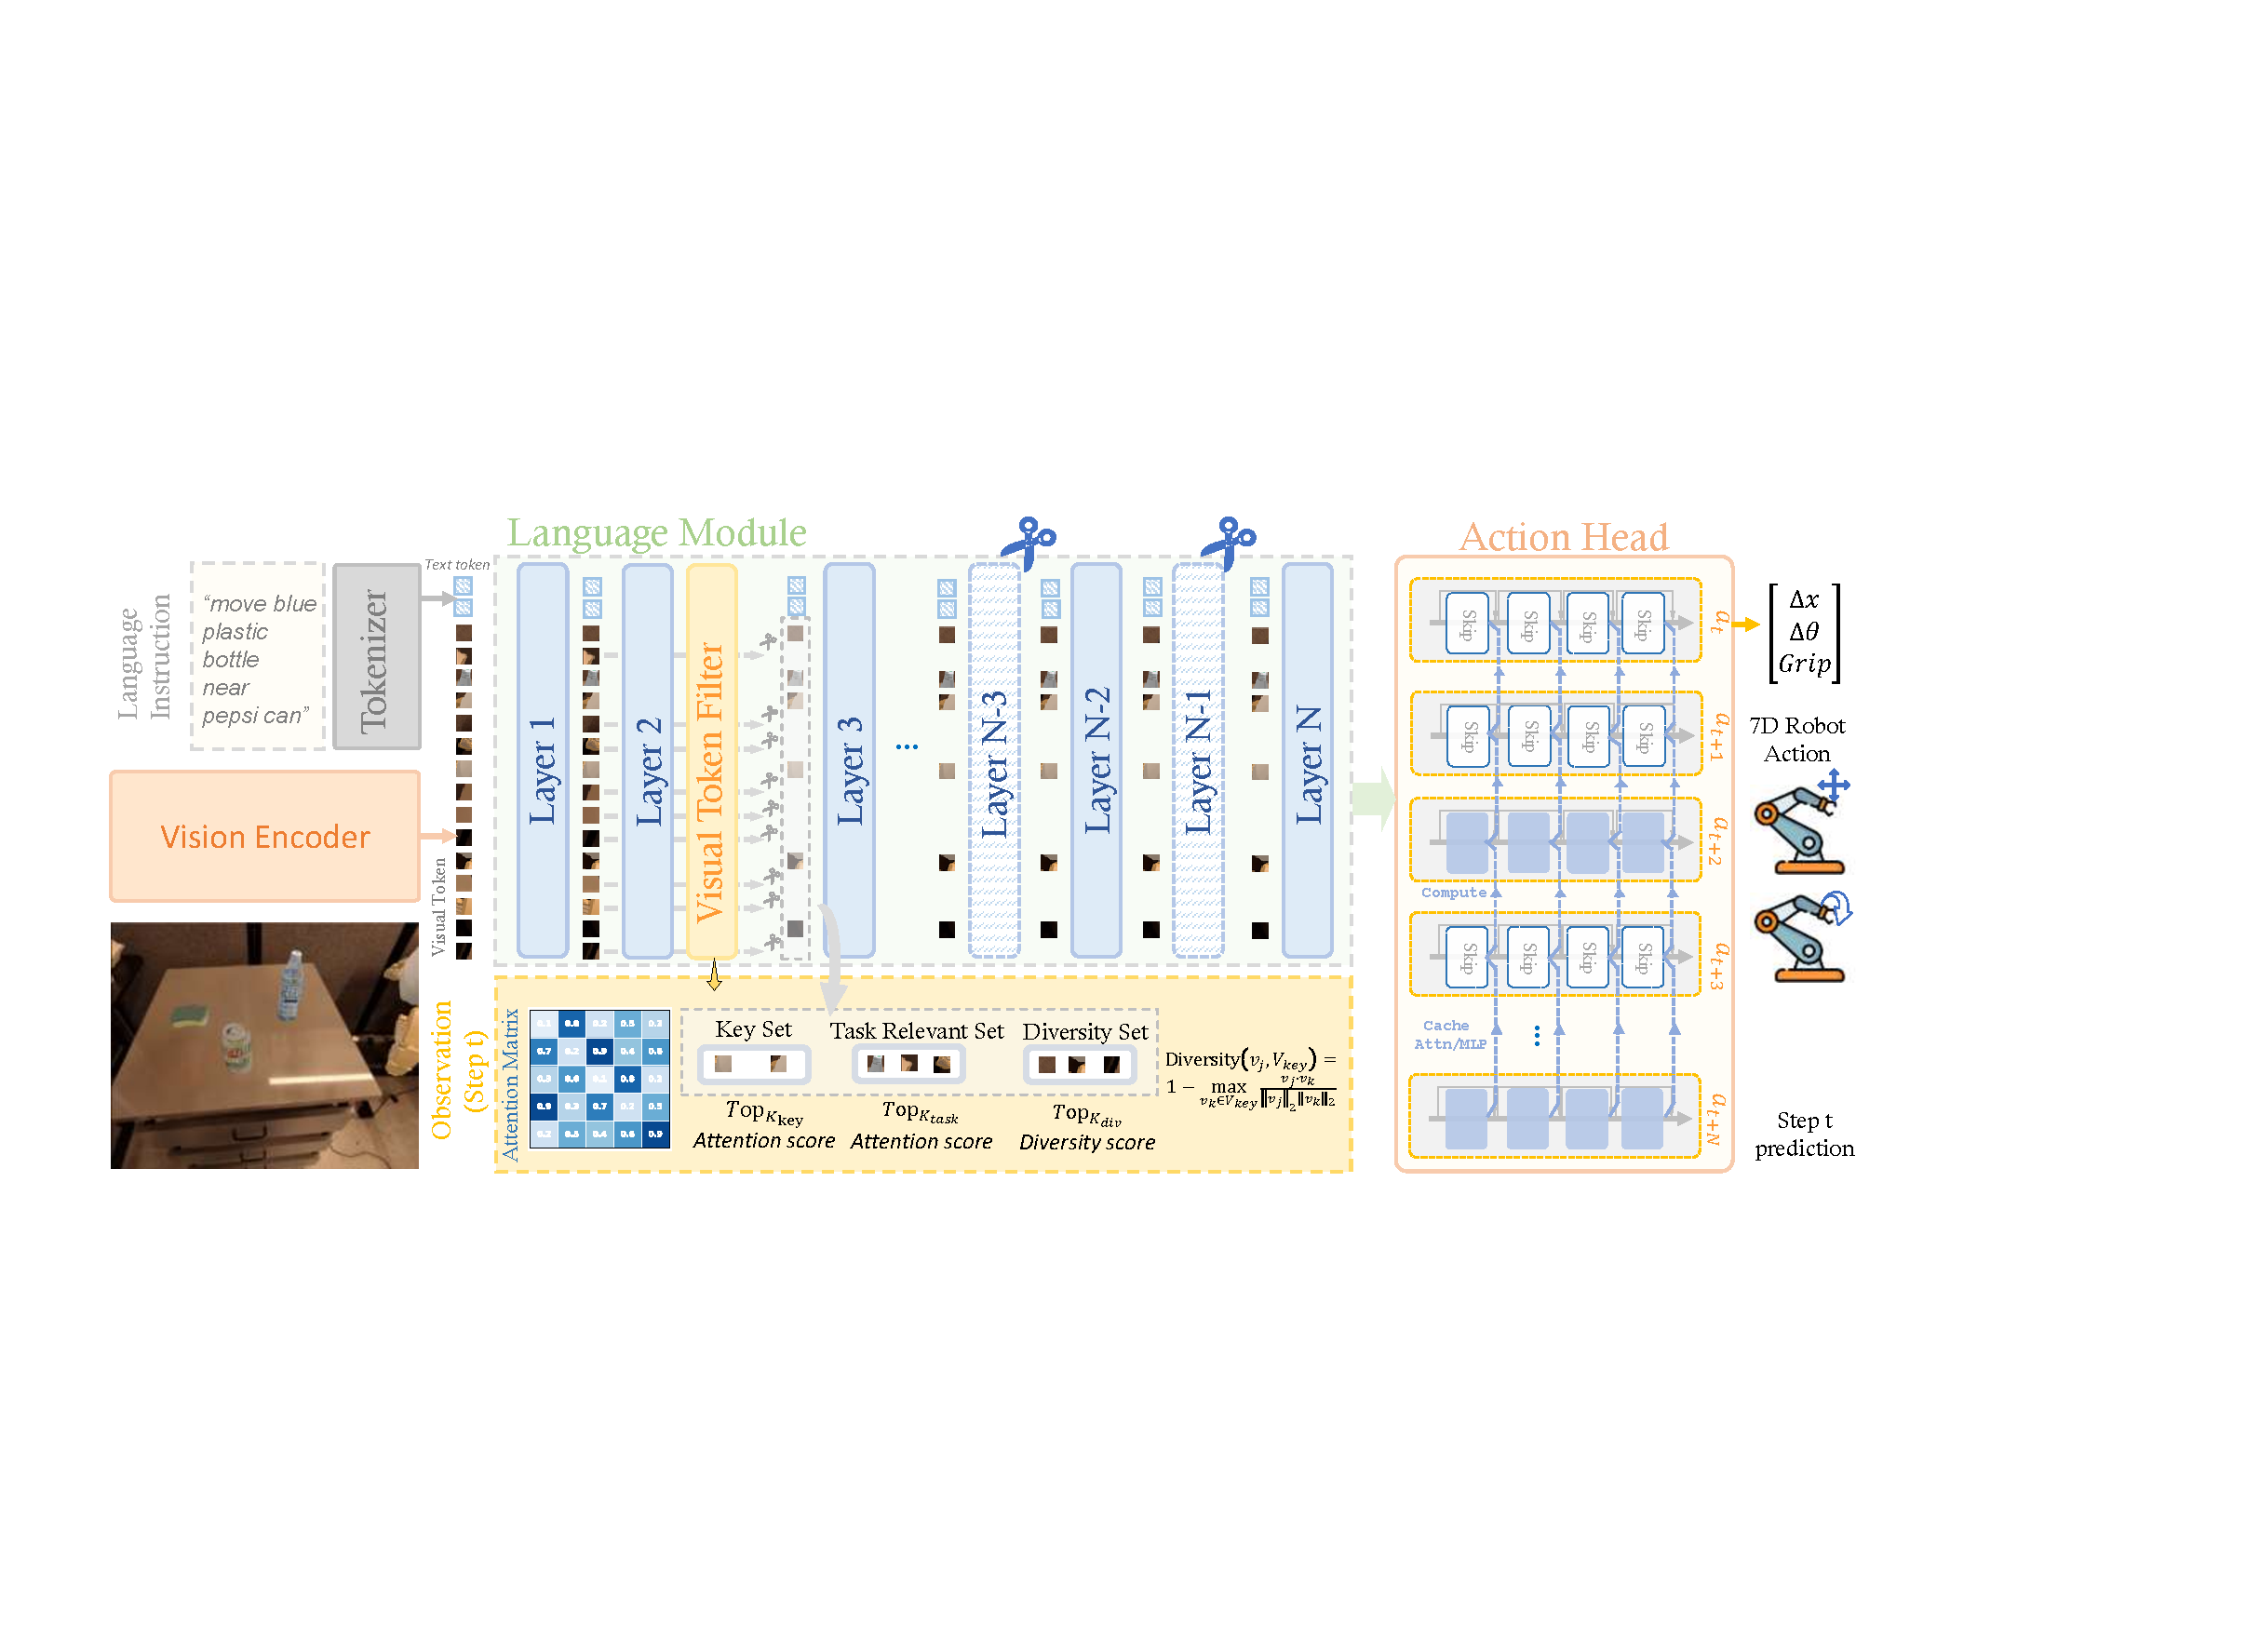
\includegraphics[width=0.99\linewidth]{figs/pipeline.pdf}
    \vspace{-5pt}
    \caption{Overview of the \textbf{\mymethod{}} framework, our training-free, structured approach to accelerate Diffusion-based VLAs. It employs: (1) pruning of redundant language module layers; (2) VLA task-aware visual token selection balancing task relevance and informational diversity; and (3) temporal caching of intermediate featuresin the diffusion action head.}
    \label{fig:pipeline}
    \vspace{-10pt}
\end{figure}


\subsection{Vision-Language Model Pruning}

\subsubsection{Layer Redundancy Analysis}


The language module within VLA models, typically a multi-layer Transformer decoder, is critical for multimodal reasoning but often introduces substantial computational overhead. Each layer $\ell$ in such a transformer updates its input hidden state $\boldsymbol{x}^{(\ell)} \in \mathbb{R}^{d \times S}$ via a residual transformation: $\boldsymbol{x}^{(\ell+1)} = \boldsymbol{x}^{(\ell)} + f(\boldsymbol{x}^{(\ell)}, \theta^{(\ell)})$, where $f(\cdot)$ is the layer-specific function with parameters $\theta^{(\ell)}$, $d$ is the hidden dimension, and $S$ is the sequence length. Our empirical analysis, illustrated in Figure~\ref{fig:bottleneck} (b), reveals significant depth-wise representational redundancy within this language module component. Specifically, we observe high cosine similarity between the input $\boldsymbol{x}^{(\ell)}$ and output $\boldsymbol{x}^{(\ell+1)}$ states for numerous, particularly deeper layers. This indicates that the effective transformation $f(\boldsymbol{x}^{(\ell)}, \theta^{(\ell)})$ imparted by these layers is minimal, rendering them functionally less critical and prime candidates for pruning to enhance inference efficiency with negligible impact on task performance. 
% 





\subsubsection{Importance-Driven Non-Contiguous Layer Pruning}

To address the identified depth-wise redundancy within the language module of VLA models, we first rigorously quantify the functional importance of each layer. Our approach aims to identify layers that contribute minimally to the transformation of hidden state representations, rendering them candidates for pruning. We define the importance score $I^{(\ell)}$ for a given layer $\ell$ based on the principle that a layer effecting substantial change to its input is more critical than one whose output closely mirrors its input. Specifically, $I^{(\ell)}$ is quantified as one minus the average cosine similarity between its input and output hidden states across a representative dataset $\mathcal{D}$ of VLA training samples and all $L$ token positions within each sample:
\begin{equation}
I^{(\ell)} = 1 - \frac{1}{|\mathcal{D}|} \sum_{i=1}^{|\mathcal{D}|} \left( \frac{1}{L} \sum_{j=1}^L \frac{\boldsymbol{x}^{(\ell)}_{i,j} \cdot \boldsymbol{x}^{(\ell+1)}_{i,j}}{\|\boldsymbol{x}^{(\ell)}_{i,j}\|_2 \|\boldsymbol{x}^{(\ell+1)}_{i,j}\|_2} \right)
\label{eq:layer_importance_score}
\end{equation}
where $\boldsymbol{x}^{(\ell)}_{i,j}, \boldsymbol{x}^{(\ell+1)}_{i,j} \in \mathbb{R}^d$ denote the input and output hidden state vectors, respectively, at position $j$ of sample $i$ for layer $\ell$. A high cosine similarity signifies a minimal transformative effect by the layer function $f(\boldsymbol{x}^{(\ell)}, \theta^{(\ell)})$, resulting in a low importance score $I^{(\ell)}$ and indicating functional redundancy.

Based on these importance scores, we employ a non-contiguous pruning strategy. For an LLM comprising $N$ layers, the importance score $I^{(\ell)}$ is computed for every layer $\ell \in \{1, \dots, N\}$. These scores are then sorted in ascending order, yielding an ordered list of layer indices $\mathcal{L}_{ranked} = [\ell_{(1)}, \ell_{(2)}, \dots, \ell_{(N)}]$ such that $I^{(\ell_{(1)})} \leq I^{(\ell_{(2)})} \leq \dots \leq I^{(\ell_{(N)})}$. Subsequently, the first $n$ layers from this list, $\{\ell_{(1)}, \ell_{(2)}, \dots, \ell_{(n)}\}$, are selected for removal from the model.




\subsection{Task-Relevance and Diversity-Driven Visual Token Pruning}



Visual token streams processed by VLA models, despite their rich informational content, frequently exhibit significant redundancy, imposing substantial computational and memory overhead. This redundancy typically manifests in two primary forms: (i) tokens possessing low relevance to the specific VLA task objectives and (ii) tokens that are informationally duplicative due to inherent visual similarities within the input. To counteract these distinct forms of superfluity, we introduce a novel, training-free, VLA task-aware visual token pruning methodology. Our approach strategically distills a compact yet maximally informative subset of visual tokens, $V_{pruned} \subset V$ of a predetermined size $K_{final}$ (from an initial set of $N_{total}$ token embeddings $V = \{v_1, v_2, \dots, v_{N_{total}}\}$ derived from the input image). This is achieved by first anchoring the selection with task-critical tokens identified via attention analysis, and subsequently augmenting this core set by judiciously balancing continued task relevance with the explicit promotion of feature diversity through similarity measures. The retained visual tokens for inference can be found in the supplementary material.



\subsubsection{Quantifying Task Relevance}


To guide visual token pruning, we quantify the task relevance for each initial visual token $v_i$ (from a set of $N_{total}$) by leveraging cross-attention scores from selected VLM layers. These scores capture the attention from $v_i$ towards $L_{ctx}$ task-defining contextual embeddings (e.g., language instructions). Let $A^{(h)}_{i,j}$ denote the attention from visual token $v_i$ to the $j^{th}$ contextual token in the $h^{th}$ attention head (of $H$ total heads). The raw task relevance score $r_i$ for $v_i$ is computed by first averaging attention contributions across all $H$ heads for each visual-contextual pair $(i,j)$, and then summing these averaged attentions over all $L_{ctx}$ contextual elements:
\begin{equation}
    r_i = \sum_{j=1}^{L_{ctx}} \left( \frac{1}{H} \sum_{h=1}^{H} A^{(h)}_{i,j} \right)
    \label{eq:task_relevance_score_concise}
\end{equation}
These raw scores $r_i$, signifying each token's overall engagement with the task context, are subsequently normalized (e.g., via min-max scaling) to standardized scores $s_i \in [0, 1]$ for robust comparison and subsequent token selection.


\subsubsection{Selection of Key Task-Relevant Tokens}
Armed with the normalized task relevance scores $\{s_i\}$, the first phase of pruning identifies an initial set of $K_{key}$ visual tokens (e.g., $K_{key}$ empirically set between 4 and 8) that demonstrate the highest relevance to the VLA task. These tokens constitute the core and indispensable visual token set, $V_{key}$:
\begin{equation}
    V_{key} = \{ v_i \in V \mid s_i \text{ is among the top } K_{key} \text{ scores in } \{s_k\}_{k=1}^{N_{total}} \}
\end{equation}
The tokens in $V_{key}$ are unconditionally retained in $V_{pruned}$, forming a foundational scaffold of visual cues deemed essential for task comprehension and successful execution. The set of remaining candidate tokens for further consideration is denoted as $V_{rem} = V \setminus V_{key}$.

\subsubsection{Augmentative Selection Balancing Relevance and Diversity}
To supplement the core set $V_{key}$ and achieve the target final token count $K_{final}$, an additional $K_{aug} = K_{final} - K_{key}$ tokens are meticulously selected from $V_{rem}$. This crucial augmentation phase is guided by a ratio $\alpha \in [0,1]$, which orchestrates a hybrid selection strategy that concurrently promotes continued emphasis on task relevance and the introduction of informational diversity.

\paragraph{Task-Driven Augmentation.}
A fraction of the augmentation quota, specifically $K_{task} = \lfloor \alpha \cdot K_{aug} \rfloor$ tokens, is selected from $V_{rem}$ by further prioritizing tokens based on their high task relevance scores $s_i$. $V_{task}$ reinforces the task-centric nature of the pruned representation by incorporating additional tokens that, while not part of the initial $K_{key}$ elite, still exhibit strong relevance signals. These tokens are added to the selection, and the pool of remaining candidates is updated: $V_{rem} \leftarrow V_{rem} \setminus V_{task}$.

\paragraph{Diversity-Driven Augmentation.}
The remaining $K_{div} = K_{aug} - K_{task}$ tokens are selected from the updated $V_{rem}$ with the explicit objective of maximizing feature diversity relative to the key selected tokens. This step is vital for capturing a broader spectrum of visual information and mitigating inherent redundancies not addressed by task relevance alone. For each candidate token $v_j \in V_{rem}$, its dissimilarity to the set $V_{key}$ is computed. A common measure is the cosine distance, ensuring that selected tokens are distinct in the embedding space:
\begin{equation}
    \text{Diversity}(v_j, V_{key}) = 1 - \max_{v_k \in V_{key}} \frac{v_j \cdot v_k}{\|v_j\|_2 \|v_k\|_2}
    \label{eq:dissimilarity}
\end{equation}


The $K_{div}$ tokens from $V_{rem}$ exhibiting the highest dissimilarity scores (i.e., those maximally different from already selected tokens) are chosen to form the set $V_{div}$. This targeted inclusion of diverse tokens ensures the final selection is not overly specialized and retains a richer contextual understanding.

\paragraph{Final Pruned Visual Token Set.}
The comprehensive set of visual tokens retained after pruning is the union of these strategically selected components:
\begin{equation}
    V_{pruned} = V_{key} \cup V_{task} \cup V_{div}
\end{equation}
This final set $V_{pruned}$, of cardinality $K_{final}$, is subsequently utilized for all downstream processing within the VLA model. This systematic reduction in visual sequence length significantly alleviates computational demands while preserving critical task-specific and diverse visual information. 

\subsection{Caching Intermediate Features in Action Prediction}

Generating high-fidelity action sequences with Diffusion-based VLA models involves an iterative denoising process that demands significant computation due to repeated self-attention and MLP computations over $T$ timesteps. We observe strong temporal coherence in the intermediate features produced during action generation (Figure~\ref{fig:bottleneck} (c)), indicating substantial redundancy across timesteps. To address this inefficiency and accelerate the action generation phase, we propose a static caching mechanism. This strategy periodically recomputes and caches critical intermediate attention and MLP output at a fixed interval $N$, reusing these cached values for the intervening time steps in the generation of action sequences. This selective computation aims to significantly reduce the computational cost associated with generating the action sequence while preserving its quality.



\subsubsection{Feature Generation and Temporal Coherence in DiT Blocks}

Let $t$ denote the current denoising timestep, typically iterating from an initial $T_{start}$ down to $1$. Within each DiT block at timestep $t$, the input features $\mathbf{z}_t$ (which may incorporate cognitive features $\mathbf{f}_t$ from upstream VLM modules and the current noise estimate) are processed sequentially by a self-attention module and an MLP module to produce intermediate hidden states:
\begin{align}
\mathbf{h}_t^{\text{attn}} &= \text{Self-Attn}(\mathbf{z}_t) \label{eq:h_attn_comp_split} \\
\mathbf{h}_t^{\text{mlp}} &= \text{MLP}(\mathbf{h}_t^{\text{attn}}+\mathbf{z}_t) \label{eq:h_mlp_comp_split}
\end{align}
These features, $\mathbf{h}_t^{\text{attn}}$ and $\mathbf{h}_t^{\text{mlp}}$, are fundamental to the denoising capacity of the diffusion model. Our observation of their high temporal coherence—meaning $\mathbf{h}_t^{\text{module}} \approx \mathbf{h}_{t-1}^{\text{module}}$ for many $t$ and module types—motivates their periodic caching and reuse.

\subsubsection{Static N-Step Caching Implementation}

We define a cache interval $N$ ($1 \le N < T_{start}$). At the initial timestep $t=T_{start}$, the features $\mathbf{h}_{T_{start}}^{\text{attn}}$ and $\mathbf{h}_{T_{start}}^{\text{mlp}}$ are computed via Equations \ref{eq:h_attn_comp_split} and \ref{eq:h_mlp_comp_split} and stored in a persistent cache, denoted $\mathcal{C}_{attn}$ and $\mathcal{C}_{mlp}$. For any subsequent timestep $t < T_{start}$, these features are recomputed and the caches are updated if and only if $t \pmod N = 0$ (assuming $t>0$ and $t$ aligns with desired multiples for caching, e.g., $T_{start}, T_{start}-N, T_{start}-2N, \dots$). Thus, for such recomputation timesteps:
\begin{align}
\mathcal{C}_{attn} &\leftarrow \text{Self-Attn}(\mathbf{z}_t) \label{eq:cache_update_attn_split} \\
\mathcal{C}_{mlp} &\leftarrow \text{MLP}(\mathcal{C}_{attn}+\mathbf{z}_t) \label{eq:cache_update_mlp_split} 
\end{align}
And the outputs for this step are $\mathbf{h}_t^{\text{attn}} = \mathcal{C}_{attn}$ and $\mathbf{h}_t^{\text{mlp}} = \mathcal{C}_{mlp}$. In all other timesteps, where $t \pmod N \neq 0$, the computationally intensive Self-Attn and MLP operations are entirely bypassed. Instead, the required features are directly retrieved from the most recently populated cache:
\begin{align}
\mathbf{h}_t^{\text{attn}} &\leftarrow \mathcal{C}_{attn} \quad (\text{when } t \pmod N \neq 0) \label{eq:cache_reuse_attn_method_split} \\
\mathbf{h}_t^{\text{mlp}} &\leftarrow \mathcal{C}_{mlp} \quad (\text{when } t \pmod N \neq 0) \label{eq:cache_reuse_mlp_method_split}
\end{align}
This static caching schedule effectively prunes the execution of these core modules for $N-1$ out of every $N$ timesteps post-initialization, leading to a substantial reduction in floating-point operations and latency for the action generation component of the VLA. The choice of $N$ allows for a tunable trade-off between acceleration and the fidelity of the generated actions, as reusing features for longer intervals might introduce slight deviations if underlying representations were to change rapidly.
